\documentclass{article}
\usepackage{graphicx} % Required for inserting images

\usepackage{cite} % 推荐加上

\usepackage{xeCJK}
\setCJKmainfont{SimSun} % 设置中文字体(Mac 下宋体,可改为 SimSun, KaiTi, PingFang SC 等)
\setmainfont{Times New Roman} % 英文正文字体
\setsansfont{Arial}          % 英文无衬线字体
\setmonofont{Courier New}    % 英文等宽字体

% 数学公式
\usepackage{amsmath, amssymb, amsfonts}
\usepackage{algorithm}      % 提供 algorithm 环境
% \usepackage{algorithmic}    % 提供 algorithmic 环境(行号、\State 等)
\usepackage{algpseudocode} % 替代 algorithmic,更现代,支持 \State、\For、\Comment

% 图形与表格
\usepackage{graphicx}
\usepackage{booktabs}
\usepackage{caption}
\renewcommand{\figurename}{图}

\usepackage{booktabs}
\usepackage{multirow}
\usepackage{array} % For the l{...} column type


\usepackage{subcaption}

% 页面设置
\usepackage[margin=2.5cm]{geometry}
\linespread{1.5} % 行距


\title{DFA-SAGE: A Dual-Fusion Aggregation Graph Sampling and Embedding Model for Enhanced Link Prediction}
\author{Desong Lin}
\date{September 2025}

\begin{document}

\maketitle

\section{Introduction}

物联网(IoT)已广泛部署于工业、医疗保健和智能家居等各类领域,为用户提供了无与伦比的便利。然而,随着物联网设备数量的持续增长,针对物联网网络的攻击也变得愈发频繁和复杂 \cite{7123563}。网络攻击者利用物联网设备固有的资源限制和安全漏洞执行恶意活动,例如分布式拒绝服务(DDoS)攻击、网络欺骗和恶意软件传播,这对用户隐私和设备可靠运行构成了重大风险,从而对物联网系统的安全性带来了显著挑战。

网络入侵检测系统(Network Intrusion Detection Systems, NIDS)是防御物联网网络攻击的关键技术,它能够及时检测设备间的异常通信和未授权访问。基于特征的入侵检测系统(Signature-based IDS)通过匹配已知攻击特征实现较低的误报率,但难以检测新型攻击 \cite{electronics9101565}。相比之下,基于行为的系统能够识别未知攻击,其中机器学习技术通过构建模型分析复杂、多维数据以实现异常检测 \cite{Hazman2023} \cite{Al-Ambusaidi2024}。尤其是深度学习方法,在自动特征提取方面表现出色,并在处理高维复杂数据方面具有卓越性能 \cite{9796521} \cite{Hanafi2024} \cite{Saravanan2024}。然而,现有基于机器学习和深度学习的 NIDS 方法通常依赖于平面数据结构提取流量特征,这限制了其捕捉物联网数据中固有空间拓扑信息的能力 \cite{10258187},从而降低了在物联网环境中的检测效果。

随着图神经网络(Graph Neural Networks, GNNs)的出现,越来越多的研究将其引入入侵检测领域 \cite{ZHONG2024103821}。GNN 主要通过信息聚合和节点更新学习节点和图的特征表示,从而能够有效建模复杂的网络结构,并捕捉图中节点间的关系。这使得 GNN 在物联网环境中具有明显优势 \cite{sanchez-lengeling2021a}。例如,GCN-Ensemble 融合模型 \cite{Mittal2024} 将流量数据转化为图结构,并整合卷积神经网络集成进行分类。这一方法有效解决了物联网入侵检测中数据不平衡和拓扑信息不足的问题,在多个数据集上取得了优异性能。在基于 GNN 的研究中,常用的图构建方法是将流量数据中的源地址和目标地址映射为图节点,而将网络流特征映射为边。然而,该方法将 IP 地址中包含的空间拓扑信息转化为图的拓扑结构,使节点本身缺乏内在特征。一些研究通过将节点特征初始化为元素全为 1 的向量,但这些特征仍缺乏区分性。此外,尽管 GNN 擅长捕捉流量数据中的复杂关系,许多方法仍主要关注节点特征的聚合与表示学习,或仅在图构建和基本权重调整阶段使用边特征。这种方法忽视了边特征在反映流量模式和捕捉攻击行为中的潜力,未能充分发挥其在图结构学习中的作用。

为了应对物联网(IoT)入侵检测的挑战,本文提出了用于物联网入侵检测的 Dual-Fusion Aggregation GraphSAGE (DFA-SAGE) 模型。

在图构建阶段,我们引入了一种基于邻近边特征聚合的节点初始化方法,利用邻接边的信息为每个节点提供独特的特征,从而增强其表达能力,克服传统方法中节点特征无效的问题。

在消息聚合过程中,我们采用双步融合聚合机制(Dual-Fusion Aggregation):
第一步(边特征强化):执行一次基于边特征的消息传递,用于强化局部边信息并初始化下一轮节点特征。

第二步(节点-边混合融合):执行第二次聚合,同时聚合上一轮更新的节点特征和原始边特征,并采用独特的自强化节点更新函数(例如,对聚合后的邻居特征进行相加操作)来深度融合特征表示。
通过独特的双步聚合操作,模型能够在单层 GNN 中有效捕获二跳邻域的边特征,从而强化局部结构信息,同时显著降低多层堆叠带来的计算复杂度和过度平滑风险。此外,在边嵌入阶段,模型保留原始边特征并与节点特征结合,采用特征缩放和相加的非线性预测,以进一步增强边特征在捕捉流量模式和攻击行为中的潜力。

总之,本文主要有三方面贡献:

1. 提出基于邻接边特征聚合的节点初始化方法: 我们提出了一种基于邻接边特征聚合的节点初始化方法,通过整合邻接边的信息赋予每个节点独特特征,从而增强其表达能力,并解决传统图构建方法中节点特征无效的问题。

2. 设计高效的双步融合聚合机制 (Dual-Fusion Aggregation): 在消息聚合阶段,我们设计了 DFA-SAGE 的双步聚合机制:第一步强化边特征,第二步融合边和节点特征,并采用独特的自强化节点更新规则。这种机制使得通过单次 DFA-SAGE 层的聚合操作即可有效获取二跳邻域的边特征,同时缓解了多层 GNN 带来的过度平滑问题,保持了模型的计算效率。

3. 验证模型的高性能和潜力: DFA-GraphSAGE 模型在 CICIoT2023、Edge-IIoT 和 BoT-IoT 数据集上表现出色,准确率和 F1 值始终高于 98.6\%,显著优于现有方法,体现了其在物联网入侵检测中的巨大潜力。

本文结构如下:第 2 节回顾了利用图神经网络进行物联网入侵检测的相关工作;第 3 节详细介绍了相关的图神经网络的研究背景,并介绍了 GraphSAGE 方法;第 4 节全面说明了所提出的 DFA-GraphSAGE 方法;第 4 节展示实验设置并分析实验结果;第 5 节总结研究并归纳关键发现。



\section{Related Work}

Haitao 等人 \cite{He2019} 设计了一种多模态序列网络入侵检测系统(NIDS),采用分层渐进网络来捕捉网络数据的不同层级特征。该方法结合了深度自编码器与 LSTM 架构,以整合相似网络连接间共享的结构信息与时间信息。该系统在三个数据集上进行了评估,包括 UNSW-NB15 数据集,在二分类实验中实现了 96.8\% 的准确率,在多分类实验中实现了 86.2\% 的准确率。

在\cite{Mu2020} 中,提出了一种针对物联网网络的攻击缓解框架,结合了基于特征与基于入侵的检测系统。基于特征的模块使用黑名单源数据库,而基于入侵的模块采用极端梯度提升(XGBoost)算法。XGBoost 分类器在 BoT-IoT 数据集上实现了 99.99\% 的二分类准确率和 0.05\% 的误报率,多分类 F1 值为 97\%,准确率为 99.96\%。

Sarhan\cite{Sarhan2021} 等人 将 UNSW-NB15、BoT-IoT 和 ToN-IoT 数据集从其原有格式及特征集合转换为统一的基于 Netflow 的格式,选择八个 Netflow 特征作为公共特征集。相应的新 Netflow 数据集(NF-UNSW-NB15、NF-BoT-IoT 和 NF-ToN-IoT)已公开发布。作者在这三个数据集上评估了 Extra Tree 集成分类器,在二分类任务中 F1 值分别为 0.85、0.97 和 1.00;在多分类任务中,对应 F1 值分别为 0.98、0.77 和 0.60。

在\cite{Kumar2020} 中,作者针对医疗物联网(IoMT)网络提出了一种两层入侵检测模型。第一层使用决策树(DT)、朴素贝叶斯(NB)和随机森林(RF)作为第一层的独立学习器;第二层采用 XGBoost 分类器对正常与攻击实例进行识别。该集成模型在 ToN-IoT 数据集上的二分类准确率为 96.35%,F1 值为 0.95。

Churcher 等人 \cite{s21020446} 应用了多种机器学习算法,包括 K 最近邻(KNN)、决策树(DT)、支持向量机(SVM)、朴素贝叶斯(NB)、随机森林(RF)、人工神经网络(ANN)以及逻辑回归(LR)进行网络入侵检测。作者在 BoT-IoT 数据集上评估了不同分类器的性能,结果显示 KNN 分类器在多分类任务中表现最佳,F1 值为 0.99,分类准确率为 99.00%。

Xiao 等人 \cite{Xiao2020}  提出了一种基于图嵌入的方法对网络流进行入侵检测。作者首先将网络流转换为一阶图和二阶图。一阶图从单个主机的角度,通过 IP 地址和端口号学习潜在特征;二阶图则从全局角度,通过源 IP、源端口、目标 IP 以及目标端口学习潜在特征。提取的图嵌入与原始特征结合后,用于训练随机森林分类器进行网络攻击检测。

然而,该方法的一个显著局限在于使用了传统的传递性图嵌入方法 \cite{hamilton2018inductiverepresentationlearninglarge},这限制了其对训练阶段未见过的图节点(如新的 IP 地址和端口号)样本的分类能力,因此不适用于大多数实际 NIDS 场景。*相比之下,本文提出的 E-GraphSAGE 方法采用归纳学习(inductive learning)策略,不存在上述限制*。

Zhou 等人 \cite{zhou2020automatingbotnetdetectiongraph}  提出使用图卷积神经网络(GCN)进行 P2P 僵尸网络节点检测。作者首先生成混合了真实大规模网络流量的僵尸网络流量,然后应用 GCN 进行节点分类。所生成的图不包含任何流或节点特征,该方法仅考虑网络连通性图的拓扑信息进行 P2P 僵尸网络节点分类,而非流分类。这限制了对僵尸网络攻击的检测,并未关注其他网络攻击(如 XSS 和勒索软件攻击),也未充分利用网络流数据中的所有信息,即网络流特征。

尽管一些现有图表示学习方法已经考虑了边特征,但没有一种可以直接应用于网络入侵检测。方法如 \cite{gong2019exploitingedgefeaturesgraph} \cite{gilmer2017neuralmessagepassingquantum} 考虑了边特征,但仅用于提升节点表示以提高性能,而非进行边分类(NIDS 的目标)。

与相关研究相比,我们的方法利用了可从网络流数据中提取的边特征,这对于通过边嵌入方法检测单独攻击流至关重要。基于传统(非图)机器学习算法的 NIDS 尚未充分利用网络流数据中固有的结构和拓扑信息来检测复杂网络攻击(如僵尸网络攻击),而这是 GNN 的关键优势。本文提出的 E-GraphSAGE 的核心创新点在于其同时利用网络流数据中的拓扑信息和边特征。此外,相关研究在 NIDS 的评估中通常仅使用 1-3 个基准数据集,而本文的方法使用了四个不同的基准数据集,提供了更高的可靠性,并验证了方法在不同网络场景下的泛化能力。

\section{Background}

\subsection{Graph Neural Network (GNN)}

GNN 是机器学习中最新的和发展最快的子领域之一。 它的强大和潜力在于它能够利用在现实世界应用领域中遇到的许多数据的固有图结构,例如社交媒体网络、生物学、电信等。 图格式通过对一组对象及其关系进行建模来捕获结构信息。 对象由图节点表示,它们的关系由图边表示。 在计算机网络的情况下,单个主机 (IP 地址) 被建模为图节点,主机之间的通信,即网络流,被建模为图边。

使用 GNN 用于 NIDS 的主要动机是能够轻松直接地利用网络流数据中丰富的结构信息,这些信息可以直接编码在图格式中。 虽然一些传统的基于 ML 的方法试图使用图数据,但这通常非常繁琐,并且依赖于手工设计的特征。

GNN 执行的常见任务是生成节点 嵌入 \cite{cai2018comprehensivesurveygraphembedding},其目标是将节点编码为低维向量,同时保持它们在原始格式中的关键关系和图位置。 节点嵌入通常是应用于下游任务(例如节点分类和节点聚类)的关键前奏 \cite{cai2018comprehensivesurveygraphembedding}。 GNN 最近因其令人信服的性能和通过可视化节点 嵌入 \cite{zhou2021graphneuralnetworksreview} 获得的结果的高度可解释性而受到广泛关注。

\subsection{GraphSAGE}

Graph Sample and AggreGatE(GraphSAGE)算法是最著名的图神经网络(GNN)之一,由 Hamilton 等人提出 \cite{hamilton2018inductiverepresentationlearninglarge},这限制了其对训练阶段未见过的图节点(如新的 。在 GraphSAGE 中,会对邻居节点进行固定大小的(均匀随机)采样。这种方式可以限制算法的空间和时间复杂度,使其不依赖于图结构(例如节点度分布)和批处理大小。

GraphSAGE 算法运行在一个图$\mathcal{G(V, E)}$上,其中 $\mathcal{V}$ 是节点集合,$\mathcal{E}$ 是边集合。节点 $v$ 的特征向量表示为 $x_v$,所有节点特征向量的集合表示为 $\{x_v, \forall v \in V\}$。

GraphSAGE 的一个关键超参数是 \textit{图卷积层数 K},它决定了在每次迭代中,节点信息聚合所能传播的跳数。另一个重要的方面是选择一个可微分的聚合函数$AGG_k,\forall k \in \{1,\cdots,K\}$,用于从邻居节点聚合信息。

该算法包括前向传播和反向传播两个阶段,下面进行更详细的说明。

类似于卷积神经网络(CNN)中的卷积操作,GraphSAGE 会收集节点局部邻域的信息,并用来计算节点嵌入。GraphSAGE 假设模型已经训练完成,即权重矩阵和聚合函数参数是固定的。
对于每个节点,算法会迭代地从节点的邻居、邻居的邻居,依次向外采样并聚合信息。
在每一层迭代中,首先会对节点的邻域进行采样,然后将采样节点的信息聚合成一个向量。在第 $k$ 层时,节点 $v$ 的邻域 $N_v$ 的聚合信息 $h_{N(v)}^k$ 可表示为公式 \eqref{eq:node-embedding-aggregation} \cite{Kumar2020}:

\begin{equation}
 h_{N(v)}^k=AGG_k (\{h_u^{k-1},\forall u \in N(v)\})
 \label{eq:node-embedding-aggregation}
\end{equation}

其中,$h_u^{k-1}$ 表示节点 $u$ 在上一层的嵌入。这些邻居节点的嵌入会被聚合到节点 $v$ 在第 $k$ 层的嵌入中。

这个聚合过程如图\ref{fig:graph-aggration}所示,展示了从每个节点的 $k$-跳邻域收集并聚合的图拓扑信息和节点特征。


\begin{figure}[h]
    \centering
    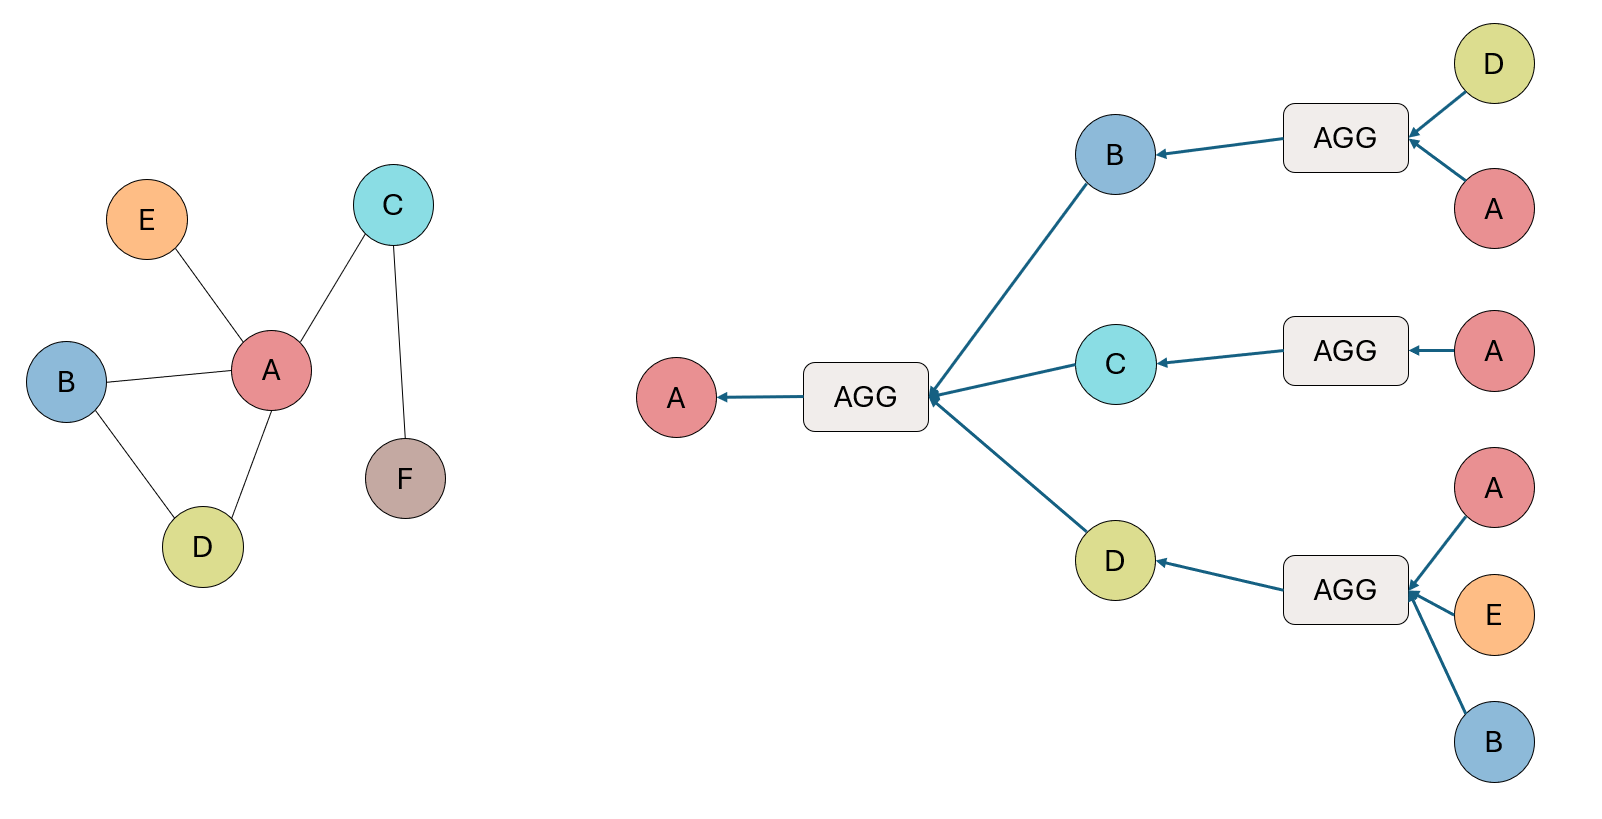
\includegraphics[width=0.6\linewidth]{images/graph-aggration.png}
    \caption{GraphSAGE 类型的消息传递和聚合机制示意图。 左侧为输入图,右侧展示了目标节点 A 如何通过聚合其一跳邻居 B、C、D 汇集的消息来更新其特征。该流程揭示了信息从二跳邻域向中心节点 A 的流动过程}
    \label{fig:graph-aggration}
\end{figure}

在 GraphSAGE 模型中,可以使用不同的聚合方法,包括均值(mean)、池化(pooling)或者不同类型的神经网络,例如长短期记忆网络(LSTM)\cite{hamilton2018inductiverepresentationlearninglarge}。

采样邻域的聚合嵌入 $h_{N(v)}^k$ 会与节点在上一层的嵌入 $h_v^{k-1}$ 进行拼接(concatenate)。然后,将模型的可训练参数 $W^k$(可训练权重矩阵)作用于拼接结果,并通过非线性激活函数 $\sigma$(例如 ReLU),即可计算第 $k$ 层节点 $v$ 的嵌入,公式如下 \cite{hamilton2018inductiverepresentationlearninglarge}:

\begin{equation}
 h_v^k=\sigma ( W_k \cdot CONCAT (h_v^{k-1},h_{N(v)}^k) )
\end{equation}

节点 $v$ 的最终表示(嵌入)记为$z_v$,即第 K 层节点的嵌入,如\eqref{eq:final-node-embedding} 所示。对于节点分类任务,$z_v$ 可以再通过 sigmoid 或 softmax 层进行输出。

\begin{equation}
 z_v=h_v^K, \forall \in V
 \label{eq:final-node-embedding}
\end{equation}
\section{Methodology}

\subsection{Dual-Fusion Aggregation SAGE (DFA-SAGE) Model}

为解决传统 GNNs 在物联网(IoT)入侵检测中节点特征无效和边特征融合不足的问题,本文提出了 \textbf{Dual-Fusion Aggregation GraphSAGE (DFA-GraphSAGE)} 模型。DFA-GraphSAGE 在 GraphSAGE 的基础上引入了\textbf{双步聚合机制}和\textbf{自强化更新函数},以深度融合节点和边特征,并强化特征的表达能力。模型的整体结构、算法流程、以及核心组件的细节详述如下。


\subsubsection{Graph Construction and Initial Feature Mapping}
% 此处描述了数据的输入和初始化,对应了代码中的输入维度设定。

图 $\mathcal{G}(\mathcal{V}, \mathcal{E})$ 由网络地址作为节点($\mathcal{V}$)和网络连接作为边($\mathcal{E}$)构建。初始的节点特征 $\mathbf{h}_v^{(0)}$ 被设置为一个与边特征维度对齐的\textbf{全一向量}(作为后续 \textbf{基于边特征的初始化} 的占位符),即 $\mathbf{h}_v^{(0)} \in \mathbb{R}^{d_{e}}$。边特征 $\mathbf{e}_{uv}$ 包含原始流量属性。根据代码($d_{e}$),所有节点和边的初始特征维度保持一致。

\subsubsection{DFA-GraphSAGE Architecture} 
% 新增部分:模型总览,对应代码中的 Model 类。

DFA-SAGE 的整体架构采用典型的 GNN-Predictor 范式,由 \textbf{Dual-Fusion Aggregation (DFA) Layer} 和 \textbf{Feature Scaling Edge Classifier} 两个核心模块串联而成。DFA Layer (对应代码中的 \texttt{SAGE} 模块) 负责通过双步消息传递学习增强的节点嵌入 $\mathbf{h}_v^K$。随后,Feature Scaling Edge Classifier (对应代码中的 \texttt{FullyConnectedPredictor} 模块) 使用这些嵌入进行最终的边分类。模型的整体信息流如图 \ref{fig:overall_architecture} 所示。

% 建议在此处放置图 1 的占位符,展示整个模型的端到端架构(输入 -> GNN -> Classifier -> 输出)。
\begin{figure}[H]
    \centering
    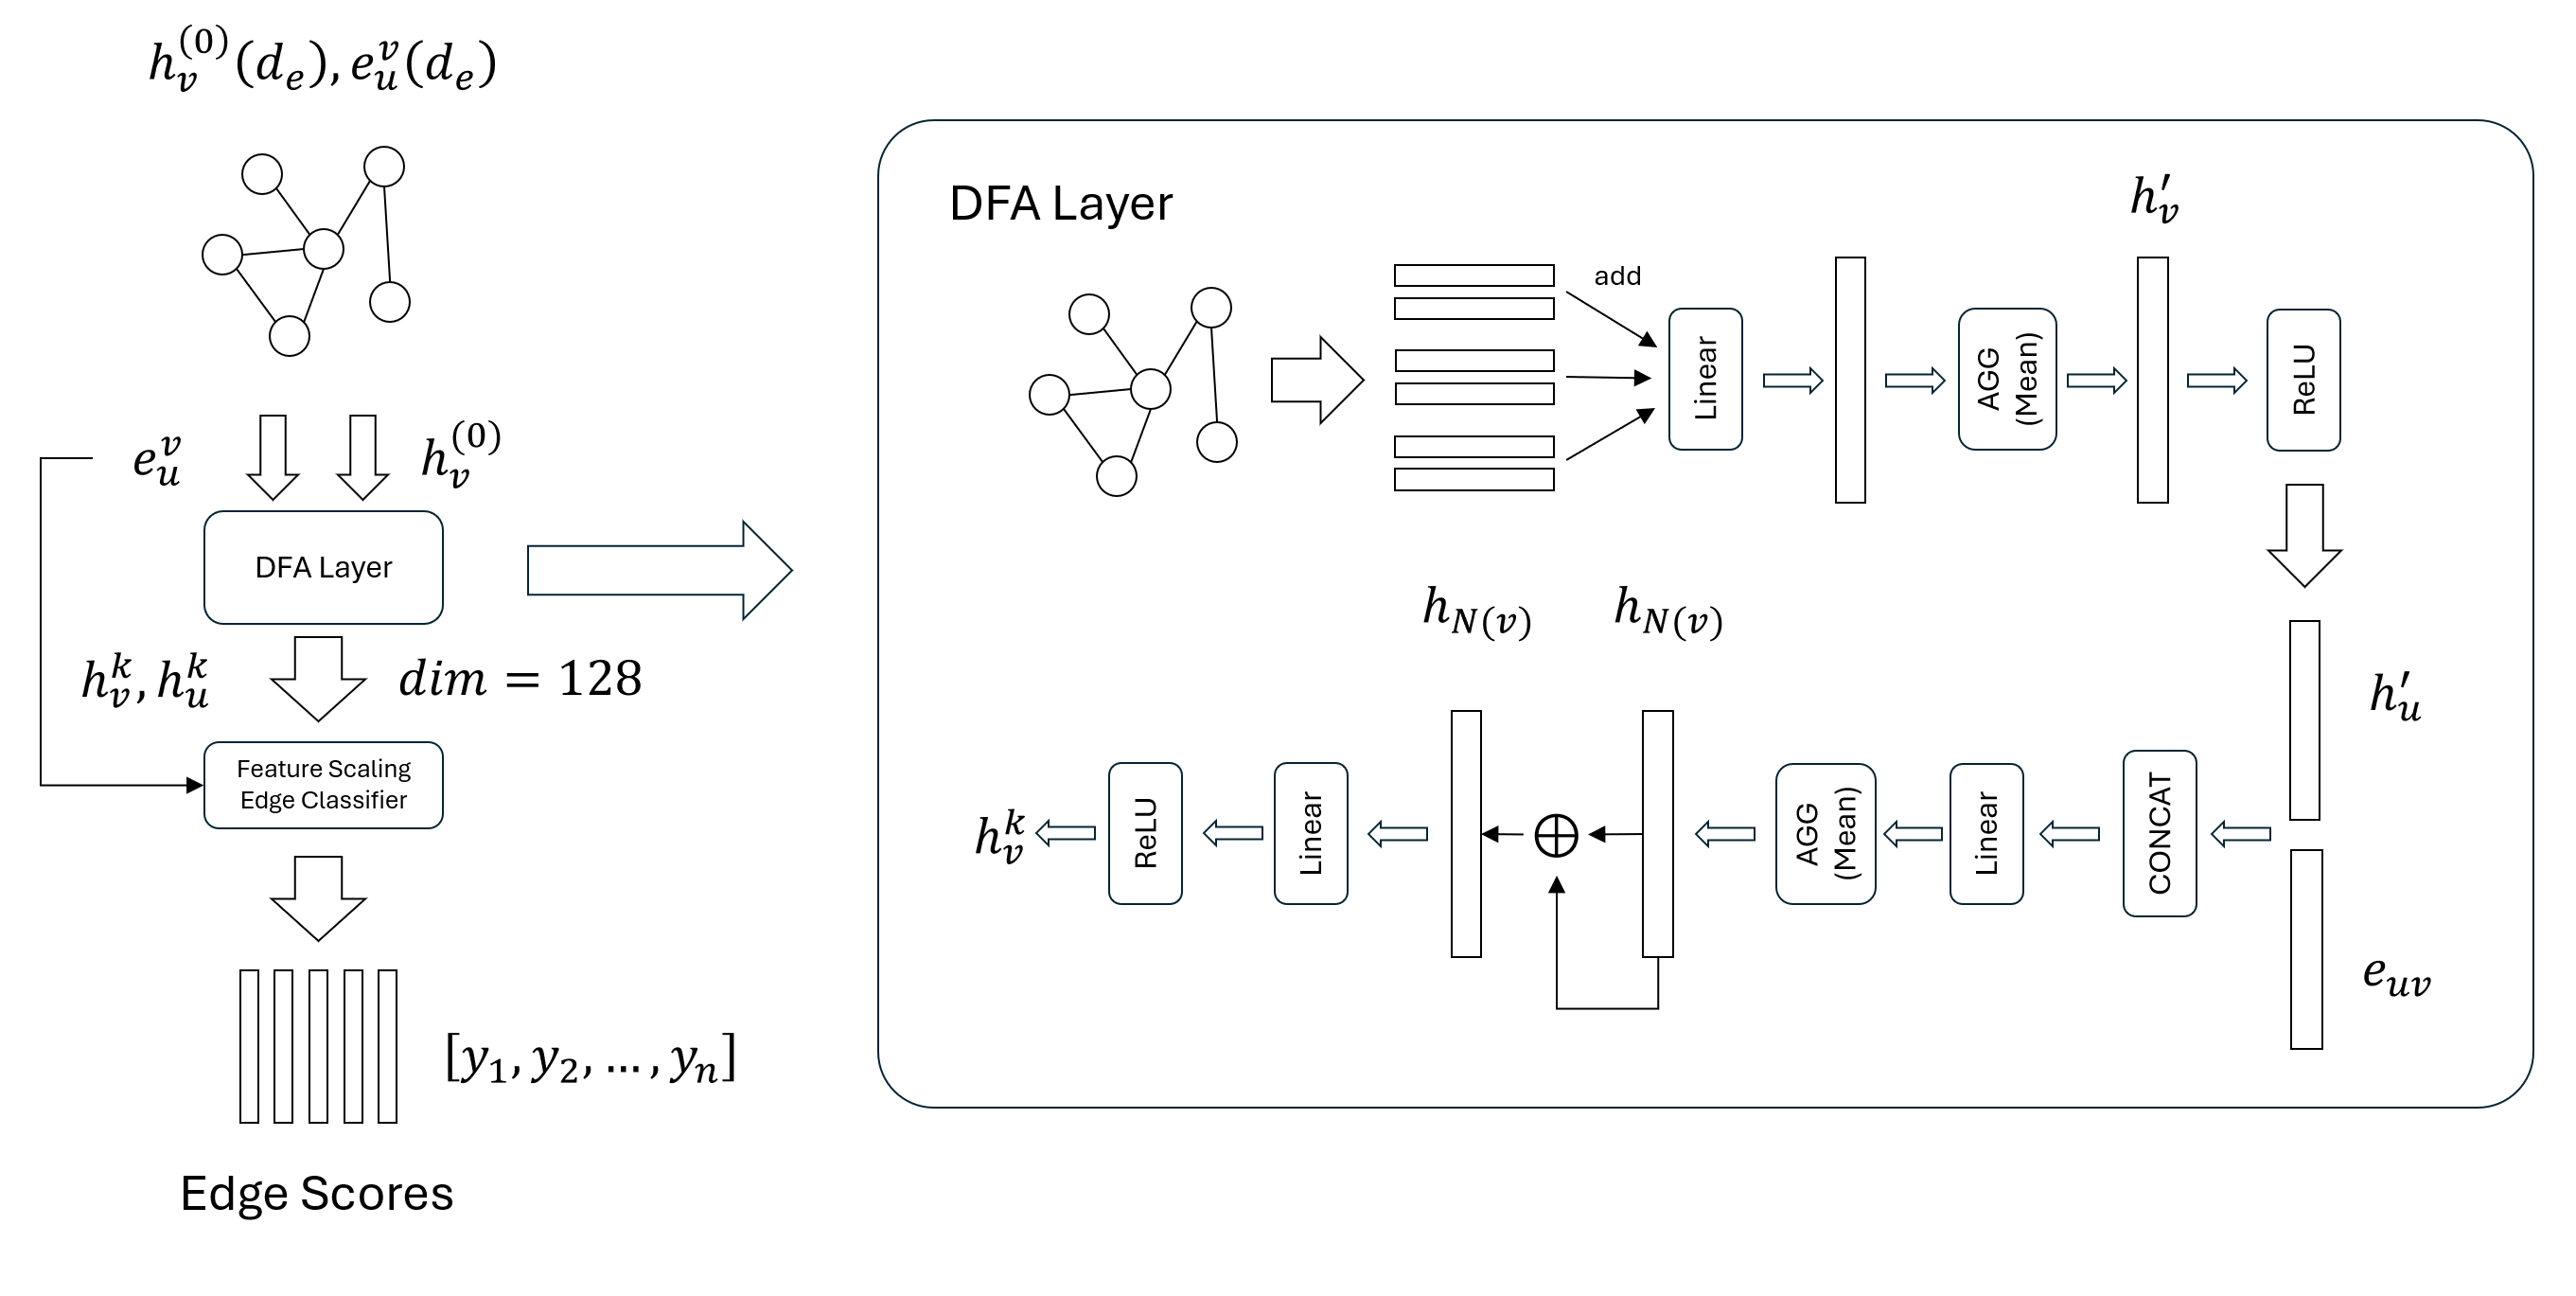
\includegraphics[width=\textwidth]{images/DFA-SAGE-architecture.png}
    \caption{DFA-SAGE 整体架构图。}
    \label{fig:overall_architecture}
\end{figure}

\subsubsection{Dual-Fusion Aggregation Layer (DFA Layer)}
% 此处描述了 GNN 核心组件 SAGELayer 的逻辑。

DFA-SAGE 的核心在于其\textbf{单层双步聚合}设计(对应代码中的 \texttt{SAGELayer}),这使其在不增加网络深度的情况下,实现对边特征的深度提取和融合。在第 $k$ 层迭代中,聚合过程分为两个连续步骤:

\begin{algorithm}
\caption{Dual-Fusion Aggregation GraphSAGE (DFA-GraphSAGE)}
\label{alg:dfa-sage}
\begin{algorithmic}[1]
\Require Graph $\mathcal{G}(\mathcal{V}, \mathcal{E})$ \Comment{节点和边集合}
\Require Input features $\mathbf{X}_{\mathcal{V}}$ \Comment{节点特征}
\Ensure Edge scores $\mathbf{Y}_{\mathcal{E}}$ \Comment{每条边分类概率}

\State $\mathbf{h}_v^{0} \leftarrow \mathbf{x}_v, \quad \forall v \in \mathcal{V}$ \Comment{节点初始化(全一向量)}
\For{$k=1$ to $K$} \Comment{GNN 迭代}
    \State // \textbf{第一步:边特征强化 (Edge Feature Reinforcement)}
    \For{$v \in \mathcal{V}$ do}
        \State $\mathbf{m}_{vu}^{(1)} \leftarrow \sigma(\mathbf{W}_{1} \cdot \mathbf{e}_{uv}), \quad \forall u \in \mathcal{N}(v)$
        \State $\mathbf{h}_v' \leftarrow \sigma(\text{AGG}(\{\mathbf{m}_{vu}^{(1)}\})) $ \Comment{更新节点特征 $\mathbf{h}'$}
    \EndFor
    
    \State // \textbf{第二步:节点-边混合融合与自强化更新}
    \For{$v \in \mathcal{V}$ do}
        \State $\mathbf{h}_{\mathcal{N}(v)} \leftarrow \text{AGG}(\{\sigma(\mathbf{W}_{msg} \cdot \text{CONCAT}(\mathbf{h}_u', \mathbf{e}_{uv})) \mid u \in \mathcal{N}(v)\})$
        \State $\mathbf{h}_v^k \leftarrow \sigma(\mathbf{W}_{apply} \cdot (\mathbf{h}_{\mathcal{N}(v)} + \mathbf{h}_{\mathcal{N}(v)}))$ \Comment{核心:邻居特征自强化}
    \EndFor
\EndFor

\State // \textbf{边预测 (Edge Prediction)}
\For{$uv \in \mathcal{E}$ do}
    \State $\mathbf{e}'_{uv} \leftarrow \sigma(\mathbf{W}_{edge} \cdot \mathbf{e}_{uv})$
    \State $\mathbf{z}_{node} \leftarrow 10 \cdot (\mathbf{h}_u^K + \mathbf{h}_v^K)$ \Comment{核心:特征缩放和相加}
    \State $\mathbf{z}_{uv} \leftarrow \text{CONCAT}(\mathbf{z}_{node}, \mathbf{e}'_{uv})$
    \State $\mathbf{y}_{uv} \leftarrow \text{Softmax}(\mathbf{W}_{pred} \cdot \mathbf{z}_{uv} + \mathbf{b})$
\EndFor

\State \textbf{return} $\mathbf{Y}_{\mathcal{E}}$
\end{algorithmic}
\end{algorithm}

\paragraph{Edge Feature Reinforcement}

该步骤旨在利用纯边特征 $\mathbf{e}_{uv}$ 生成一个强化后的边上下文信息,并更新节点特征。这确保了节点特征 $\mathbf{h}_v^{(k)}$ 在随后的聚合中,起始就融入了高质量的局部边信息。

\textbf{消息函数 $\phi_1$ 和更新 $\gamma_1$:}
$$
\mathbf{m}_{vu}^{(1)} = \sigma \left( \mathbf{W}_{1} \cdot \mathbf{e}_{uv} \right)
$$
\begin{equation}
\mathbf{h}_v' = \sigma \left( \underset{u \in \mathcal{N}(v)}{\text{AGG}} (\mathbf{m}_{vu}^{(1)}) \right)
\end{equation}

其中 $\mathbf{W}_{1}$ 是可训练的线性矩阵,负责将边特征投影到消息空间。$\mathbf{h}_v'$ 是第一次聚合后的节点特征,它将作为第二次聚合中节点 $\mathbf{h}_v$ 的输入。

\paragraph{Node-Edge Hybrid Fusion with Self-Reinforcement}

该步骤执行最终的消息聚合,将第一次更新的节点特征 $\mathbf{h}_u'$ 与原始边特征 $\mathbf{e}_{uv}$ 融合,并采用独特的\textbf{自强化更新函数}。

\textbf{消息函数 $\phi_2$:}
$$
\mathbf{m}_{vu}^{(2)} = \sigma \left( \mathbf{W}_{msg} \cdot \text{CONCAT}(\mathbf{h}_u', \mathbf{e}_{uv}) \right)
$$

\textbf{自强化更新 $\gamma_2$:}
聚合的邻居信息 $\mathbf{h}_{\mathcal{N}(v)}$ 可表示为:
$$
\mathbf{h}_{\mathcal{N}(v)} = \underset{u \in \mathcal{N}(v)}{\text{AGG}} (\mathbf{m}_{vu}^{(2)})
$$

最终的节点嵌入 $\mathbf{h}_v^{(k)}$ 通过自强化机制计算,如公式 \eqref{eq:dfasage-update} 所示:
\begin{equation}
\mathbf{h}_v^{(k)} = \sigma \left( \mathbf{W}_{apply} \cdot (\mathbf{h}_{\mathcal{N}(v)} + \mathbf{h}_{\mathcal{N}(v)}) \right)
\label{eq:dfasage-update}
\end{equation}

其中,$\mathbf{W}_{msg}$ 和 $\mathbf{W}_{apply}$ 均为可训练权重矩阵。这里的 $\mathbf{h}_{\mathcal{N}(v)} + \mathbf{h}_{\mathcal{N}(v)}$ 是一种\textbf{邻居特征自强化(Self-Reinforcement)}操作,旨在通过放大邻居信息的影响,加速特征的学习和传播,有效增强浅层 GNN 的特征表达能力。

% 建议在此处放置图 2 的占位符,展示 DFA Layer 内部的双步聚合过程和自强化机制。
% \begin{figure}[htbp]
%     \centering
%     \includegraphics[width=\textwidth]{dfa_layer_internal.png}
%     \caption{DFA Layer 内部双步聚合机制图。}
%     \label{fig:dfa_layer_internal}
% \end{figure}

\subsubsection{Feature Scaling Edge Classifier}
% 此处描述了预测器 FullyConnectedPredictor 的逻辑。

DFA-SAGE 专注于边分类任务。它采用一个全连接预测器 $\text{PRED}(\cdot)$,在最终分类之前执行非标准的特征缩放操作,以突出节点特征的重要性。

首先,对原始边特征 $\mathbf{e}_{uv}$ 进行线性转换,得到 $\mathbf{e}'_{uv}$:
\begin{equation}
\mathbf{e}'_{uv} = \sigma(\mathbf{W}_{edge} \cdot \mathbf{e}_{uv})
\end{equation}

然后,将最终节点嵌入 $\mathbf{h}_u^{(k)}$ 和 $\mathbf{h}_v^{(k)}$ 通过\textbf{特征缩放和相加}进行组合,并与 $\mathbf{e}'_{uv}$ 拼接,如公式 \eqref{eq:dfasage-prediction} 所示:

\begin{equation}
\mathbf{z}_{uv} = \text{CONCAT} \left( 10 \cdot (\mathbf{h}_u^{(k)} + \mathbf{h}_v^{(k)}), \quad \mathbf{e}'_{uv} \right)
\label{eq:dfasage-prediction}
\end{equation}

缩放因子 $10$ 旨在为 GNN 学习到的节点信息赋予更高的权重,以平衡可能过度依赖原始边特征的问题。最终的边分类分数 $\mathbf{y}_{uv}$ 通过 Softmax 函数输出:
$$
\mathbf{y}_{uv} = \text{Softmax} \left( \mathbf{W}_{pred} \cdot \mathbf{z}_{uv} + \mathbf{b} \right)
$$
其中 $\mathbf{y}_{uv}$ 即为该网络连接属于各个入侵类别的概率分布。

\section{Experiments}

\subsection{数据集}

本研究使用的实验数据集包括以下内容:

\begin{itemize}
    \item \textbf{CICIoT2023 \cite{202305.0443}}:该数据集由加拿大网络安全研究所 (CIC) 提出,是一个针对大规模攻击的实时物联网 (IoT) 数据集,包含七类攻击和正常流量的 PCAP 文件。由于硬件限制,本研究从原始 548~GB PCAP 文件中选择了部分数据作为实验数据集。采样依据原始数据集中各类别的比例进行,为解决少数类别样本不足的问题(例如 Recon 类),适当提高了其采样比例。最终,实验数据集中选取了 449,094 条记录。

    \item \textbf{Edge-IIoT \cite{9751703}}:该数据由十余种 IoT 设备生成,包含与 IoT 和 IIoT 协议相关的 14 种攻击类型。

    \item \textbf{BoT-IoT \cite{KORONIOTIS2019779}}:Koroniotis 等人 (2019) 构建的数据集,主要用于物联网相关研究。数据集包含六类攻击以及 47 个特征,并附有对应的类别标签。
\end{itemize}

各数据集的主要特征如表~\ref{tab:dataset_classes} 所示。

\begin{table}[H]
\centering
\caption{Number of the classes of the selected datasets}
\label{tab:dataset_classes}
\begin{tabular}{l c r l c r}
\toprule % 顶线
\textbf{Dataset} & \textbf{Attack} & \textbf{Count} & \textbf{Dataset} & \textbf{Attack} & \textbf{Count} \\
\midrule % 表头线

% --- CICIoT2023 (8行) & Edge-IIoT (14行) 开始 ---
\multirow{8}{*}{\centering CICIoT2023} & DoS & 96,992 & \multirow{14}{*}{\centering Edge-IIoT} & Normal & 20,111 \\
& DDoS & 77,776 & & DDoS\_ICMP & 14,090 \\
& Benign & 65,448 & & DDoS\_HTTP & 10,560 \\
& Spoofing & 58,825 & & SQL\_injection & 10,297 \\
& Mirai & 55,736 & & Uploading & 10,261 \\
& BurteForce & 38,376 & & DDoS\_TCP & 10,247 \\
& Web-based & 36,178 & & Vulnerability\_scanner & 10,062 \\
& Recon & 19,763 & & Password & 9,976 \\
% --- CICIoT2023 结束 / BoT-IoT (5行) 开始 ---
% Edge-IIoT 的 multirow 仍在继续
\multirow{5}{*}{\centering BoT-IoT} & DDoS & 534,494 & & Backdoor & 9,917 \\
& Reconnaissance & 91,082 & & Ransomware & 9,886 \\
& DoS & 42,390 & & XSS & 9,702 \\
& Normal & 477 & & Port\_Scanning & 8,992 \\
& Theft & 79 & & DDoS\_UDP & 1,402 \\
% --- 补齐 Edge-IIoT 的最后一行 ---
% \cline{5-6} % 使用 cline 来创建一条 Edge-IIoT 和 BoT-IoT 分隔线(可选,如果想保持简洁,可以去掉)
% 为了保持 BoT-IoT 和 Edge-IIoT 行数对齐,这里需要一个额外的空行来放置 Edge-IIoT 的最后一行数据
& & & & Fingerprinting & 869 \\
\bottomrule % 底线
\end{tabular}
\end{table}

\subsection{实验设置}

\subsubsection{实验环境与参数}
本实验在以下硬件与软件环境下进行:
\begin{itemize}
    \item 处理器:Intel Core i9-14900K
    \item 显卡:NVIDIA GeForce RTX 4060 Ti,16~GB 显存
    \item 内存:16~GB
    \item 操作系统:Windows~10
    \item 编程语言与框架:Python 3.10,PyTorch 2.4.0
    \item 优化器:Adam,用于训练神经网络,加速收敛到全局最优解
    \item 模型训练相关参数:表~\ref{tab:dfasage_parameters} 列出了详细参数设置
\end{itemize}

\begin{table}[H]
\centering
\caption{DFA-GraphSAGE 模型关键参数与维度 (Key Parameters and Dimensions of the DFA-GraphSAGE Model)}
\label{tab:dfasage_parameters}
\begin{tabular}{lcc}
\toprule % 顶线
\textbf{模块 (Module)} & \textbf{参数 (Parameter)} & \textbf{维度/值 } \\
\midrule % 表头线
\textbf{输入特征 (Input Features)} & 原始边特征 ($\mathbf{e}_{uv}$) 维度 & $d_e=13$ \\
& 初始节点特征 ($\mathbf{h}_v^0$) 维度 & $d_{e}=13$ (全一向量) \\
% \addlinespace % 增加小间距代替细横线
\midrule % 表头线
\textbf{DFA Layer (SAGELayer)} & 第一次聚合输出维度 & $d_{out}=128$ \\
& 第二次聚合输入 (Concat) 维度 & $128 + 13 = 141$ \\
& GNN 嵌入维度 ($\mathbf{h}_v^K$) & $128$ \\
& 消息聚合次数 ($K$) & $1$ \\
% \addlinespace % 增加小间距代替细横线
\midrule % 表头线
\textbf{特征缩放分类器 (Predictor)} & 节点特征输入维度 & $128$ \\
& 转换边特征 ($\mathbf{e}'_{uv}$) 维度 & $128$ \\
& 最终拼接 ($\mathbf{z}_{uv}$) 维度 & $128 + 128 = 256$ \\
& 节点特征缩放因子 & $10$ \\
& 输出类别数 & $\text{Num\_Classes}$ \\
\bottomrule % 底线
\end{tabular}
\end{table}

\subsubsection{评估指标}
本文采用以下指标对模型的性能进行全面评估:
\begin{itemize}
    \item \textbf{准确率 (Accuracy, ACC)}:衡量分类正确的样本占总样本的比例
    \item \textbf{精确率 (Precision, $P_c$)}:衡量模型预测为正类的样本中,实际为正类的比例
    \item \textbf{召回率 (Recall, $R_c$)}:衡量实际为正类的样本中,被正确预测为正类的比例
    \item \textbf{F1 分数 (F1-score, $F1_c$)}:精确率和召回率的调和平均,用于综合评估模型性能
\end{itemize}

其数学表达式如下:
\begin{align}
\text{准确率 (ACC)} &= \frac{TP + TN}{N} \label{eq:accuracy} \\
\text{精确率 (P}_c\text{)} &= \frac{TP_c}{TP_c + FP_c} \label{eq:precision} \\
\text{召回率 (R}_c\text{)} &= \frac{TP_c}{TP_c + FN_c} \label{eq:recall} \\
\text{F1 分数 (F1}_c\text{)} &= 2 \cdot \frac{P_c \cdot R_c}{P_c + R_c} \label{eq:f1score}
\end{align}

其中,$TP$、$TN$ 分别表示正类和负类预测正确的样本数,$FP$、$FN$ 分别表示误判的样本数,$N$ 为总样本数。
\subsection{实验结果与分析}

\subsubsection{模型性能分析}

Table X(请替换为表格编号,如 Table 5)展示了我们提出的 Dual-Fusion Aggregation SAGE (DFA-SAGE) 模型在 CICIoT2023 数据集上的多类别分类结果。

实验结果有力地证明了 DFA-SAGE 模型在多类别入侵检测任务中表现出色,其平均准确率 (Average Accuracy) 达到了 99.XX\%。模型的平均查准率 (Precision)、查全率 (Recall) 和 F1-score 均保持在 99.X\% 附近。对于大多数类别,模型的分类性能接近完美,例如 DoS 和 Mirai 类别的 F1-scores 分别达到了 99.XX\% 和 99.XX\%。然而,针对 Recon 类别,查全率略低于其他类别,为 9X.XX\%,这可能归因于该类别数据特征的复杂性或样本分布不均。

图 X(请替换为图片编号,如 Figure 5)展示了 DFA-SAGE 模型针对每个类别的 ROC 曲线。如图所示,所有类别的曲线均紧密贴近左上角,表明模型能有效地区分正负样本。图表右下角的数据显示,所有类别的 AUC 值均超过 0.9X,突显了模型在跨类别分类中优异的判别能力,充分证实了其在多类别分类任务中的高性能。

图 Y(请替换为图片编号,如 Figure 6)展示了各类别对应的 PR 曲线。大多数类别展现出强大的性能,其中 Class X、Class Y 和 Class Z(请根据您的类别代号替换)的 AUC-PR 值分别达到了 1.0000、0.99XX 和 0.96XX,说明这些类别具有高查准率和高查全率。与此形成对比的是,Class A 和 Class B(请根据您的类别代号替换)的 AUC-PR 值相对较低,分别为 0.XX 和 0.XX,这可能暗示这些类别的分类性能仍有提升空间,例如存在误分类或查全率不足的问题。总体而言,尽管 DFA-SAGE 在大多数类别上性能优异,但少数类别的分类仍有改进余地。

图 Z(请替换为图片编号,如 Figure 7)比较了 CICIoT2023 数据集在经过 DFA-SAGE 特征提取前后的 t-SNE 可视化效果。原始特征(左侧)在降维后类别边界模糊,某些类别存在明显的重叠,不利于有效区分。相比之下,经 DFA-SAGE 提取的特征(右侧)在各类别内形成了更紧凑的聚类,且类别间边界更加清晰,表明 DFA-SAGE 通过利用双步融合机制和自强化更新学习到了更具判别力的 GNN 特征。右侧图像中的局部聚类结构进一步证实,DFA-SAGE 在降维过程中有效地保留了利用节点-边关系所捕获的关键类别信息。

\paragraph{鲁棒性优化与两阶段训练策略}

在模型训练的初期探索中,我们观察到轻微的过拟合现象,推测是模型学习了过多的细节和噪声所致。为解决此问题,我们系统性地探索了三种优化策略:L2 正则化、在模型中添加 Dropout 层,以及使用调度器进行动态学习率调整(Lr-Scheduler)。实验结果(总结于 Table K,请替换为表格编号,如 Table 6)表明,Lr-Scheduler+L2 组合在权衡收敛速度、推理效率和模型尺寸方面表现最佳,因此被确定为 DFA-SAGE 第一阶段(Stage 1)训练的基础优化策略。

基于此最优基础策略,为了进一步稳定训练并达到最佳泛化性能,我们采用了两阶段训练策略:

\begin{enumerate}
\item 第一阶段(Stage 1:端到端训练): 使用 Lr-Scheduler+L2 对 DFA-SAGE 的所有参数进行训练,旨在让 DFA Layer 学习到高质量、高鲁棒性的节点嵌入$ h_v^K $。
\item 第二阶段(Stage 2:预测器精调): 在 GNN 嵌入稳定后,我们采取了参数冻结策略。冻结 DFA Layer 的所有参数,仅使用固定的低学习率 1e-4 精细调整特征缩放边分类器 ($W_pred$ 和 $W_edge$) 的参数。这一阶段有效地利用了稳定的图特征,专注于优化分类器的决策边界,并取得了最终的最佳性能。
\end{enumerate}

图 P(请替换为图片编号,如 Figure 8)展示了使用 Lr-Scheduler+L2 方法进行第一阶段训练时,训练集和验证集的损失曲线。随着 epochs 的增加,训练损失和验证损失趋于收敛,且验证损失没有出现明显的上升趋势,这表明该方法有效地缓解了过拟合。

\paragraph{泛化性验证}

为证明所提出模型强大的跨数据集鲁棒性,我们进一步使用 Edge-IIoT 和 BoT-IoT 数据集进行了验证性实验。这些实验旨在评估模型在不同 IoT 网络环境下的稳定性和可靠性。Table R(请替换为表格编号,如 Table 7)呈现了模型在三个数据集上的分类结果,而 图 Q(请替换为图片编号,如 Figure 9)展示了对应分类任务的混淆矩阵。

实验结果表明,DFA-SAGE 模型在 Edge-IIoT 和 BoT-IoT 数据集上分别取得了 9X.XX\% 和 99.XX\% 的准确率,对应的 F1-scores 分别为 9X.XX\% 和 99.XX\%。在所有三个数据集上,模型的一致性表现突出,准确率、查准率、查全率和 F1-score 均接近或超过 98\%,充分展示了 DFA-SAGE 强大的跨数据集鲁棒分类能力。
\bibliographystyle{IEEEtran}   % 或 plain, unsrt, alpha...
\bibliography{ref}             % ref.bib

\end{document}
